\setchapterpreamble[u]{\margintoc}
\chapter{Statistical Approach to Drop Formation}
\labch{dropstat}


\section{Monte Carlo Approach}



% interested in long time dynamics as coalescences lead to larger drop sizes


\section{Millimeter Scale Ensembles}

%impact of bin sizes

\subsection*{Diameter Distributions}

% short time scales


\begin{figure*}
\centering
\includegraphics{plots/drop_stats/short_time_diameter_bins.pdf}
	\caption{\blindtext}
\label{t1_dia_bins}
\end{figure*}

% long time scales


\begin{figure*}
\centering
\includegraphics{plots/drop_stats/long_time_diameter_bins.pdf}
	\caption{\blindtext}
\label{t2_dia_bins}
\end{figure*}

% PDF predictions of data at long times


\begin{figure*}
\centering
\includegraphics{plots/drop_stats/long_time_diameter_fits.pdf}
	\caption{\blindtext}
\label{t2_dia_fits}
\end{figure*}

% N^{-1/2} scaling of error 

% extrapolations of RP etc , limit of volume of largest drop

\subsection*{Volume Distributions}

% short time scale 


\begin{figure*}
\centering
\includegraphics{plots/drop_stats/short_time_volume_bins.pdf}
	\caption{\blindtext}
\label{t1_vol_bins}
\end{figure*}



% long time scale


\begin{figure*}
\centering
\includegraphics{plots/drop_stats/long_time_volume_bins.pdf}
	\caption{\blindtext}
\label{t2_vol_bins}
\end{figure*}


% PDF predictions of data at long times


\begin{figure*}
\centering
\includegraphics{plots/drop_stats/long_time_volume_fits.pdf}
	\caption{\blindtext}
\label{t2_vol_fits}
\end{figure*}

% N^{-1/2} scaling of error 


\subsection*{Influence of Corrugation Amplitude}

% temporal variation in drop size PDF's for low and high levels of corrugation

\begin{figure}
\centering
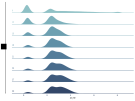
\includegraphics{plots/drop_stats/small_amp.pdf}
	\caption{\blindtext}
\label{tseries_small}
\end{figure}

\begin{figure}
\centering
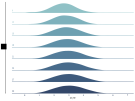
\includegraphics{plots/drop_stats/large_amp.pdf}
	\caption{\blindtext}
\label{tseries_large}
\end{figure}

% side by side comparison


\begin{figure*}
\centering
\includegraphics{plots/drop_stats/amp_dist_compare.pdf}
	\caption{\blindtext}
\label{tseries_comp}
\end{figure*}


\section{Description of Large Sizes}


% estimation of error with binomial distribution



% linear fitting, with and without uncertainty, full distribution and tail zoom  

% methodology to determine best fit

\begin{figure}
\centering
	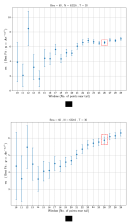
\includegraphics{plots/drop_stats/determine_fit_linear.pdf}
	\caption{\blindtext}
\label{determine_linear}
\end{figure}


% without uncertainty

\begin{figure}
\centering
\includegraphics{plots/drop_stats/linear_tail_fit_uncertainty_no.pdf} \\
\includegraphics{plots/drop_stats/linear_zoom_tail_fit_uncertainty_no.pdf} \\ 
\caption{\blindtext}
\label{linear_fits_wo}
\end{figure}

% with uncertainty

\begin{figure}
\centering
\includegraphics{plots/drop_stats/linear_tail_fit_uncertainty_yes.pdf} \\
\includegraphics{plots/drop_stats/linear_zoom_tail_fit_uncertainty_yes.pdf} \\ 
\caption{\blindtext}
\label{linear_fits_with}
\end{figure}


% log(log) vs log fitting, with and without uncertainty, full distribution and tail zoom  

% methodology to determine best fit

\begin{figure}
\centering
	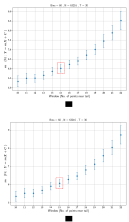
\includegraphics{plots/drop_stats/determine_fit_log.pdf}
	\caption{\blindtext}
\label{determine_log}
\end{figure}

% without uncertainty

\begin{figure}
\centering
\includegraphics{plots/drop_stats/log_tail_fit_uncertainty_no.pdf} \\
\includegraphics{plots/drop_stats/log_zoom_tail_fit_uncertainty_no.pdf} \\ 
\caption{\blindtext}
\label{log_fits_wo}
\end{figure}


% with uncertainty

\begin{figure}
\centering
\includegraphics{plots/drop_stats/log_tail_fit_uncertainty_yes.pdf} \\
\includegraphics{plots/drop_stats/log_zoom_tail_fit_uncertainty_yes.pdf} \\ 
\caption{\blindtext}
\label{log_fits_with}
\end{figure}

\subsection*{Weakly Non-Linear Theory}



% stephane's predictions and verifications


